\documentclass{article}
\usepackage[utf8]{inputenc}
\usepackage{lmodern}
\usepackage[english]{babel}
\usepackage[autostyle]{csquotes}
\usepackage{amsfonts}
\usepackage{amsmath}
\usepackage{graphicx}
\usepackage{minted}
\usepackage{float}
\usepackage[backend=biber,style=authoryear]{biblatex}
\usepackage{booktabs}
\usepackage{appendix}
\usepackage{ltablex}
% \usepackage[margin=1in]{geometry}
\addbibresource{ref.bib}

\newcommand{\argmax}[1]{\underset{#1}{\operatorname{arg}\,\operatorname{max}}\;}
 
\graphicspath{{images}}

\title{Predicting Superconductivity Critical Temperature\\
\large CS5014 Practical 1}
\author{190027392}
\date{March 2020}

\begin{document}

\maketitle
\newpage
\tableofcontents
\listoffigures
\listoftables
\listoflistings
\newpage

\section{Introduction}
\section{Loading, Splitting and Cleaning}
\paragraph{} The dataset provided is a compilation of 21,263 super conductor containing 81 attributes compiled from Japan’s National Institute for Materials Science. 
\paragraph{Splitting the dataset} The dataset was immediately split into training and testing data, the latter being discarded away for evaluation purposes. The training dataset was used during training and development of the models. This was implemented in the generate\_data.py file which returns these two split datasets.
\label{section:pipeline}
\paragraph{Pipeline} A Pipeline by SKLearn was used to automate the cleaning tasks as shown in Listing~\ref{lst:pipeline}. This would allow the training data to be cleaned up without inspecting it hence reducing the risk of Data Leakage. The Dataframe selector is a helper function designed to select only a subset of the features as to not apply this pipeline to the output feature.

\begin{listing}[ht]
\label{lst:pipeline}
\begin{minted}[linenos, breaklines]{python}
def get_pipeline(inputs) -> Pipeline:
    return Pipeline([
        ('selector', DataFrameSelector(inputs)),
        ('std_scaler', StandardScaler()),
    ])


def apply_pipeline(data, x_col, y_col):
    y = data[y_col]
    data = DataFrame(get_pipeline(x_col).fit_transform(data), columns=x_col)
    data['critical_temp'] = y
    x, y = data[x_col], data[y_col]
    return data, x, y
\end{minted}
\caption{The Pipeline for Standardising the Data}
\end{listing}{}

\section{Visualising The Data} The describe.py script plots a number of charts attempting to display the and describe the data. Due to the high number of dimensions a scatter plot with some of the most important features found later during development is shown (Figure~\ref{fig:scatter}).

\begin{figure}[H]
\label{fig:scatter}
  \centering
    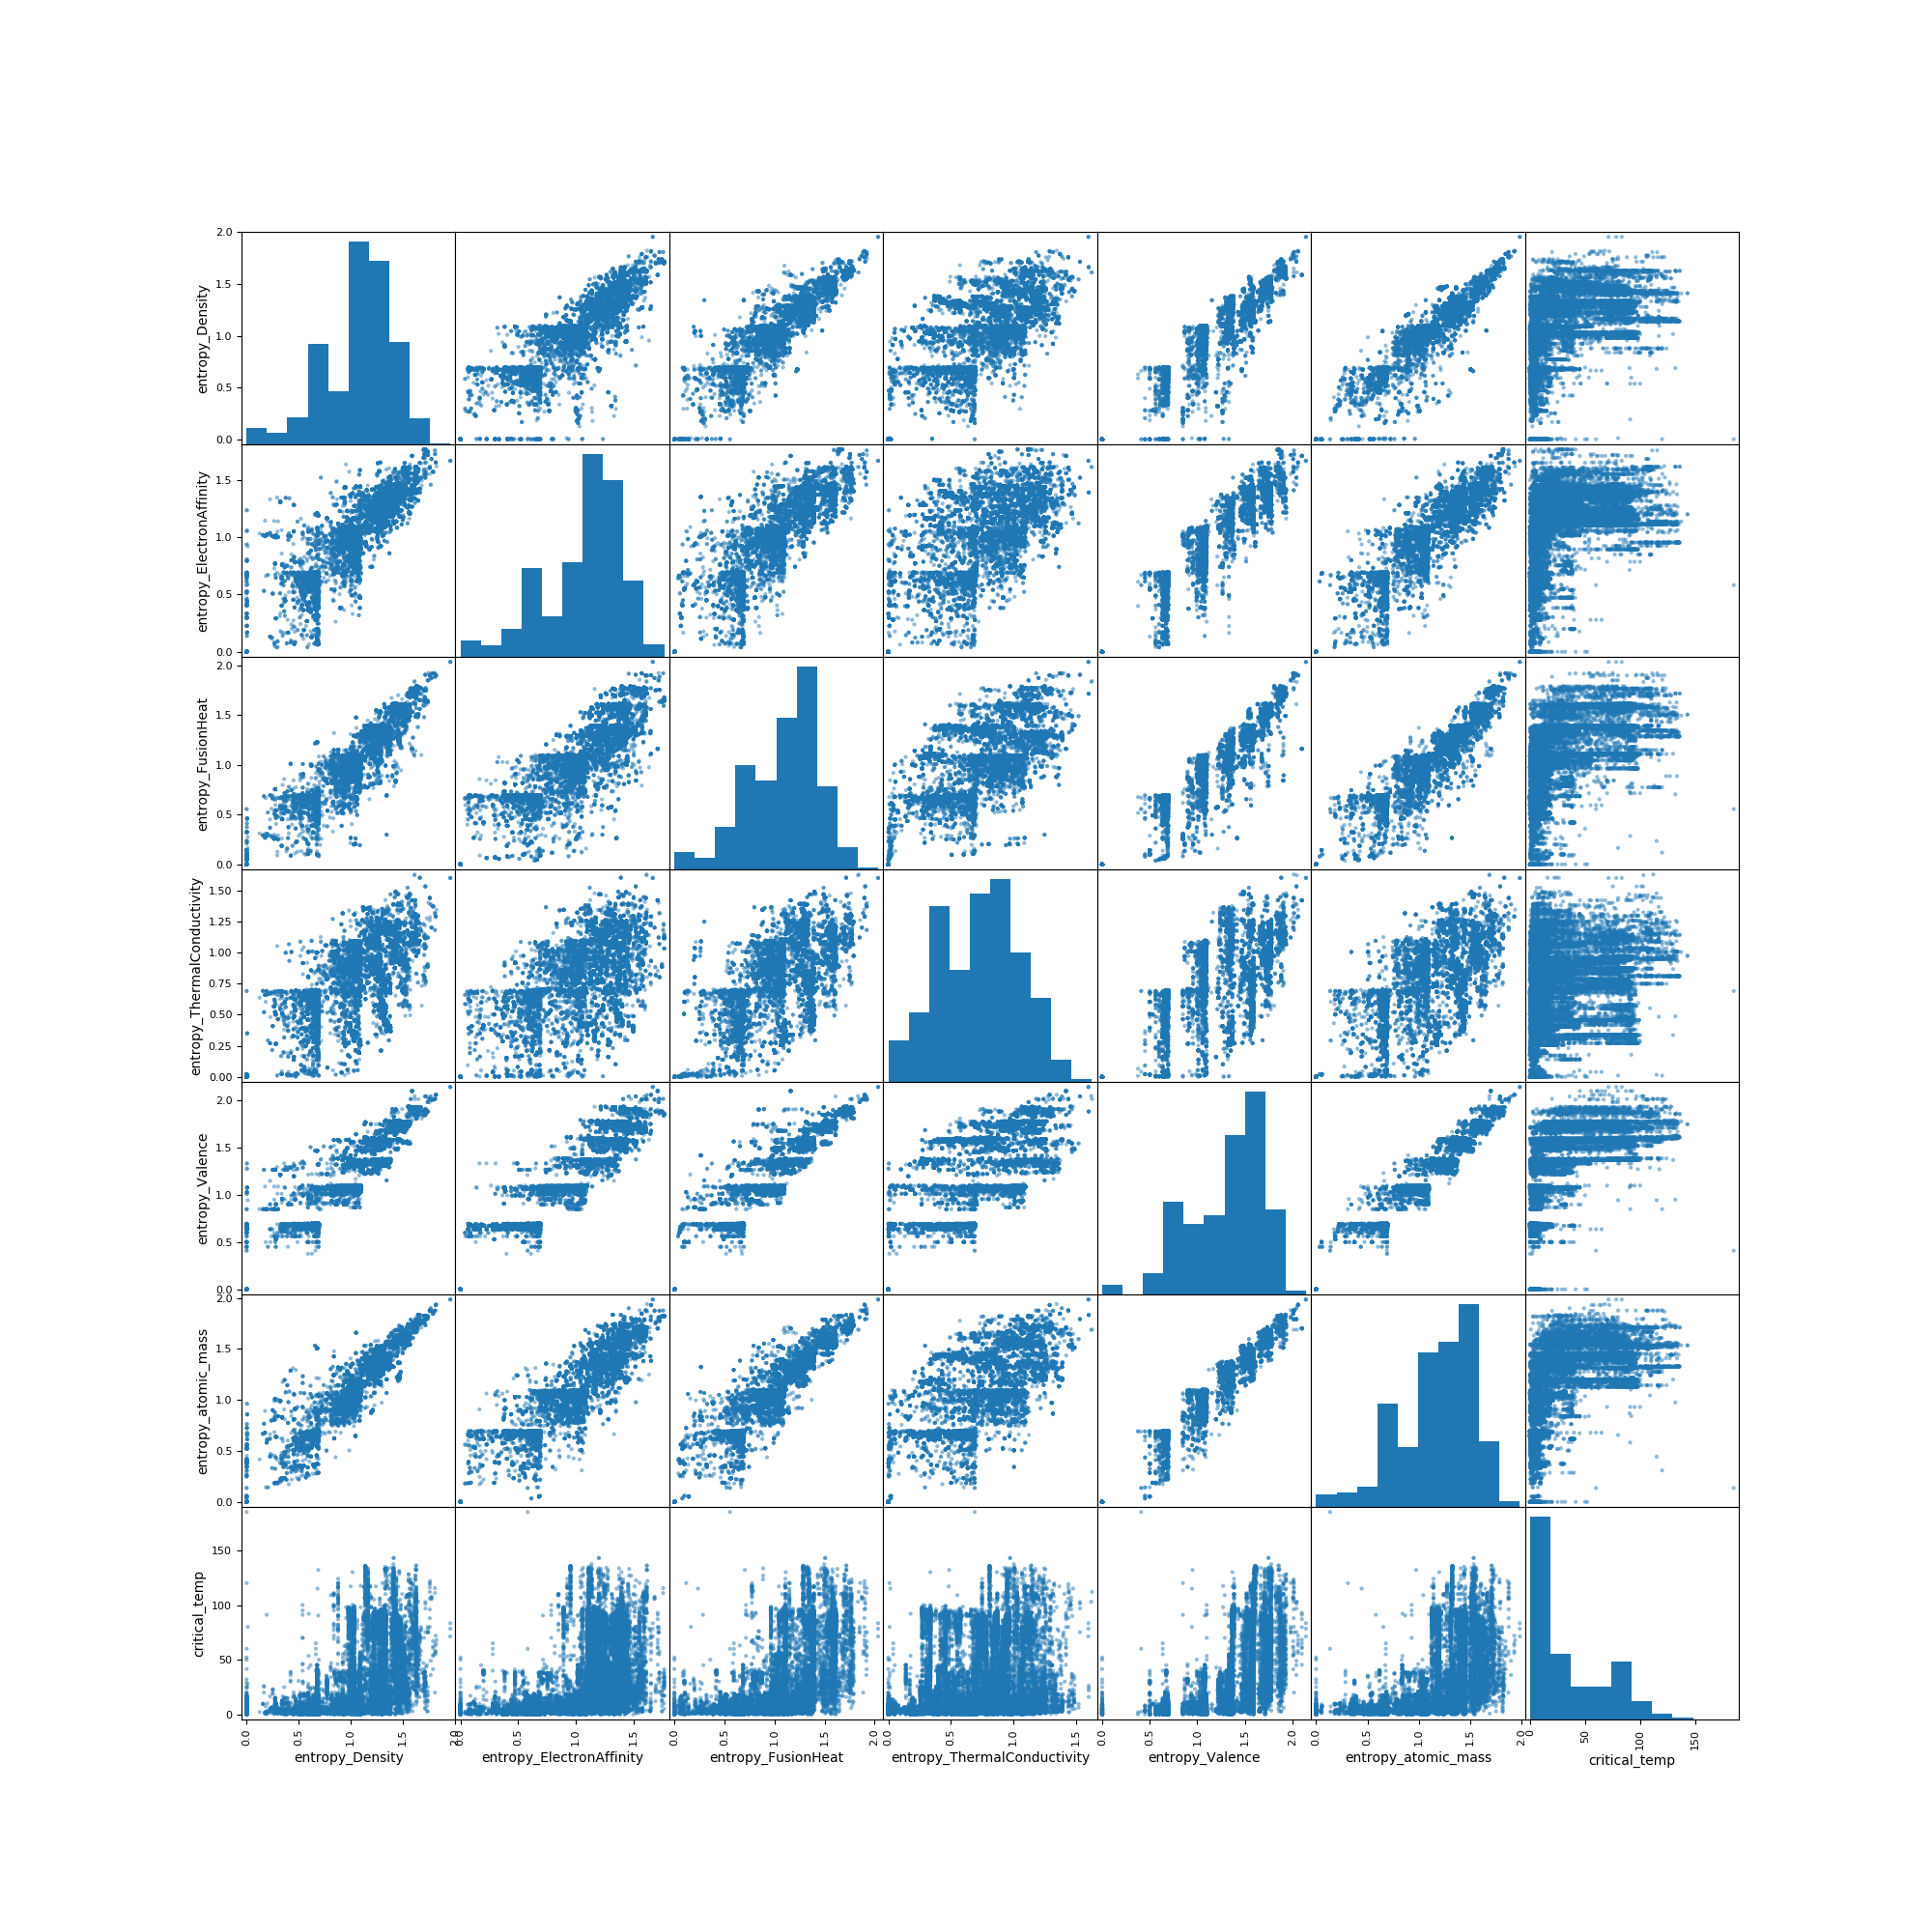
\includegraphics[scale=0.2]{images/scattermatrix.png}
    \caption{A scatter matrix showing the correlations between some of the important features.}
\end{figure}
Figure~\ref{fig:heat} gives a general brief overview of all the variables and their correlation. The map shows that the variables are highly correlated with one another as shown by the high concentrations of yellow in the matrix. As the data is so highly correlated, multicollinearity could be an issue. Multicollinearity is a statistical phenomenon occurring in multiple regression where a feature could be predicted linearly from the other features. This could lead to a situation where the coefficients of the model changing erratically with small changes in the data. Formally a set of variables are perfectly collinear when:
\begin{equation}
    0 = \lambda_1X_{1i} +\dots +\lambda_kX_{ki}
\end{equation}{} for a regression model
\begin{equation}
    Y_1 = \beta_0+\beta_1X_{1i} + \dots + \beta_kX_{ki} + \epsilon
\end{equation}{}
\begin{figure}[H]
\label{fig:heat}
  \centering
    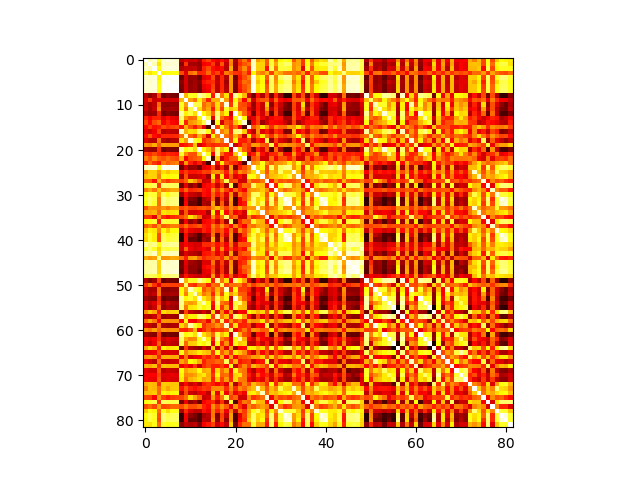
\includegraphics[scale=0.7]{images/heatmap.png}
    \caption{A heatmap of correlations. Brighter colors indicate higher correlation.}
\end{figure}


\section{Feature Reduction}
\subsection{Variance Inflation Factor} 
The Variance Inflation Factor(VIF) is a measure of colinearity of the input features in multiple regression. It is defined as:
\begin{equation}
    VIF_i = \frac{1}{1-R_i^2}
\end{equation}{}
This measure was integrated into the pipeline and the \(VIF\) for each of the columns is calculated. As a general rule columns having a score larger than 10 are removed~\autocite{kutner2005applied}.
\subsection{Principle Component Analysis}
Principle component analysis is a statistic procedure that orthogonally transforms a dataset into uncorrelated variables called principle components~\autocite{pearson1901liii}. The first principle component \(x_1\) covers the maximum possible variance in the data such that:
\begin{equation}
    w_1 = \argmax{||w||=1} \left(\sum_i t_i^2 \right) = \argmax{||w||=1}\left(\sum_i (x_i \cdot w)^2 \right)
\end{equation}{}
where \(w_k = w_1\dots 1_k\) representing the vectors of the coefficients and \(t_i\) is the vector of principle component scores. The other components could be calculated subtracting the first \(k-1\) principle components and finding the weight vectors that maximises the variance as before.

\subsection{Selecting a Feature Reduction Technique} An experiment was devised to score these techniques on the training dataset to choose the best technique for our testing. The experiment written in feature\_selection.py, spins up a cross validator, tries each of these techniques and tables up the results for comparison shown in Table~\ref{tab:featurereduction}. The dataset was standardised using the pipeline discussed in Section~\ref{section:pipeline}. This is important as PCA extracts the components that maximise the variance, hence having features of different scale might disproportionately affect the variance messing up the grouping. The results show that non of the techniques out performed the benchmark vanilla linear regression. None of the techniques managed to reduce the number of features to a manageable level indicating that most of the features are required to capture most of the variance in the dataset. As a result these techniques were abandoned as they performed worse than the vanilla linear regression. 
% Please add the following required packages to your document preamble:
% \usepackage{booktabs}
\begin{table}[]
\centering
\begin{tabular}{@{}lll@{}}
\toprule
Technique        & Cross Validation Score & Number of features \\ \midrule
Benchmark       & 0.7342                 & 80                 \\
VIF Elimination & 0.6523                 & 29                 \\
PCA             & 0.5951                 & 16                 \\ \bottomrule
\end{tabular}
\caption{Scores for the feature reduction techniques. }
\label{tab:featurereduction}
\end{table}
\section{Regression Models}
In the following section a brief explanation of the models used will be given along with regularization techniques employed.
\subsection{Linear Regression}
Linear regression is a simple linear approach to modelling the relationship between a dependent variable and it's predictors. Formally it is described as:
\begin{align}
    y_i &= \beta_0 + \beta_1x_{i1} + \dots + \beta_1x_{ip} + \epsilon_i \\
    y &= X\beta + \epsilon_i && \text{Matrix notation}
\end{align}{}
where \(y\) is a vector of outputs, \(X\) is a matrix of row vectors \(x_i\) and \(x_{i0} = 1~for~i=1,\dots,n\), \(\beta\) is a vector of coefficients and \(\epsilon\) is a vector of error terms~\autocite{hastie2009elements}. Linear regression aims to optimise \(\beta\) and \(\epsilon\) in such a way that the cost function would be minimised. The cost function could be described as:
\begin{equation}
    \sum_{i=1}^M (y_i-\hat{y_i})^2 = \sum^M_{i=1}\left(y_i-\sum^p_{j=0}w_j \cdot x_{ij}\right)^2
\end{equation}{} where \(M\) and \(p\)
\paragraph{Regularisation} Regularisation allows the model to generalise well over unseen samples in the real world. One problem of the standard linear regression is that the resulting model would be too complex. In this case linear regression would have 80 coefficients which could lead to an over-fitted model.
\paragraph{Ridge Regularisation} Here the cost function described for Linear Regression is modified in such a way that a penalty is added to coefficients of large magnitude.
\begin{equation}
    \sum_{i=1}^M (y_i-\hat{y_i})^2 = \sum^M_{i=1}\left(y_i-\sum^p_{j=0}w_j \cdot x_{ij}\right)^2 + \lambda\sum^p_{j=0}w^2_j
\end{equation}{}
\(\lambda\) refers to the penalty term. Setting this to 0 would turn this cost function into the one used by linear regression minimising this property.
\paragraph{Lasso Regularisation} Like Ridge Regularisation, Lasso builds up on the Linear Regression's cost function as follows:
\begin{equation}
    \sum_{i=1}^M (y_i-\hat{y_i})^2 = \sum^M_{i=1}\left(y_i-\sum^p_{j=0}w_j \cdot x_{ij}\right)^2 + \lambda\sum^p_{j=0}|w_j|
\end{equation}{}
It takes account the magnitudes rather than the coefficients hence leading to zero coefficients and a simpler model.
\subsection{Random Forest Regression} Random Forests is a machine learning technique built on Decision Trees. Decision Trees are sensitive on the trained data hence if the training data changes slightly the resulting model could be drastically different. They also tend to stick to local optima (no back tracing after splitting the tree) and risk over-fitting. Random Forests employ a bagging technique (random sampling with replacement) by deploying multiple decision trees in parallel and returns the mean prediction of the individual trees. Each tree samples randomly a sample on every split reducing the chances of over-fitting.
\subsection{Metrics}
\paragraph{Root Mean Square Error(RMSE)} The RMSE error for prediction \(\hat{y}_t\) and \(T\) samples is defined as:
\begin{align}
    RMSE = \sqrt{\frac{\sum^T_{t=1}(\hat{y}_t-y_t)^2}{T}}
\end{align}{} RMSE is frequently used as the error is on the same scale of the output (in our case Kelvin). Errors are squared before taking the root hence high errors are penalised.
\paragraph{\(R^2\)} the \(R^2\) error or coefficient of determination compares the resultant model with a constant baseline. The error can range from \(-\infty to 1\) where negative values indicate that the model performs worse than the baseline.
\begin{align}
    R^2 = 1- \frac{MSE(model)}{MSE(baseline)}
\end{align}{}
\section{Results and Discussion}
The evaluation script is located in the evaluate\_models.py file. The script trains a Linear Regression, Ridge regression and Random forest using a K-Fold cross validator on the training dataset and then scores these models using the RMSE and R2 metrics. The script also produces learning graphs(Figure) and residual plots of the evaluated model and saves them in the fig directory. The Lasso regression was not included as this model could not converge. This could be due to a small tolerance value for the variance of the dataset. This phenomenon was not investigated further due to time constraints. Table~\ref{tab:scores} shows the scores achieved by the models whilst Figure~\ref{fig:residual} shows the residual plots for each of the model.

\begin{table}[]
\centering
\begin{tabular}{@{}lll@{}}
\toprule
Model             & Mean Square Error & R2   \\ \midrule
Linear regression & 17.38             & 0.73 \\
Ridge Regression  & 17.9              & 0.72 \\
Random Forest     & 11.96             & 0.88 \\ \bottomrule
\end{tabular}
\caption{Scores for the trained models}
\label{tab:scores}
\end{table}

\begin{figure}[H]
\label{fig:residual}
  \centering
    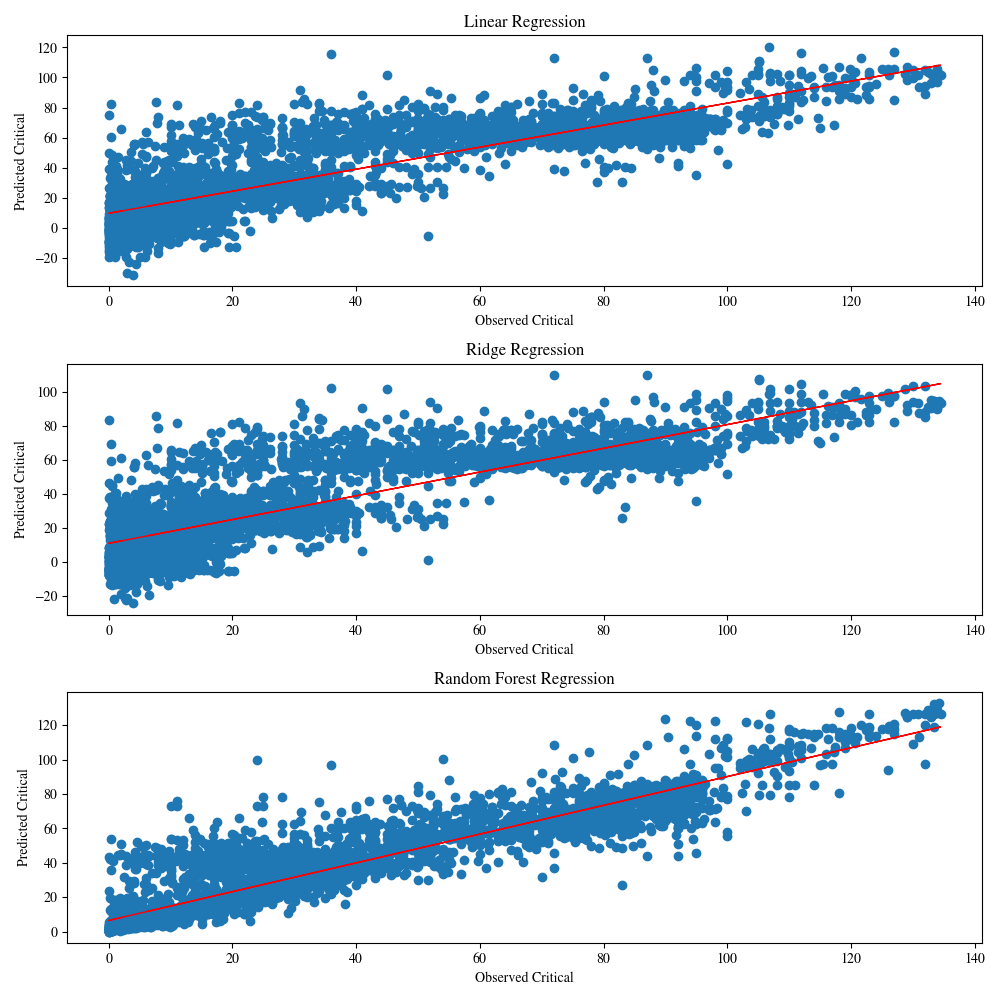
\includegraphics[scale=0.55]{images/residual.png}
    \caption{A matrix of residual plots of the different models.}
\end{figure}

These results coincide with the results obtained in the original paper where the RMSE obtained was 17.6 K. and a \(R^2\) of 0.74~\autocite{hamidieh2018data}. The Ridge model is also close to the score obtained by the original paper. The XGBoost Model described in the paper also out-performs the Random Forest Regressor as it obtains a RSME of 9.5 K.

\begin{figure}[H]
\label{fig:learningcurve}
  \centering
    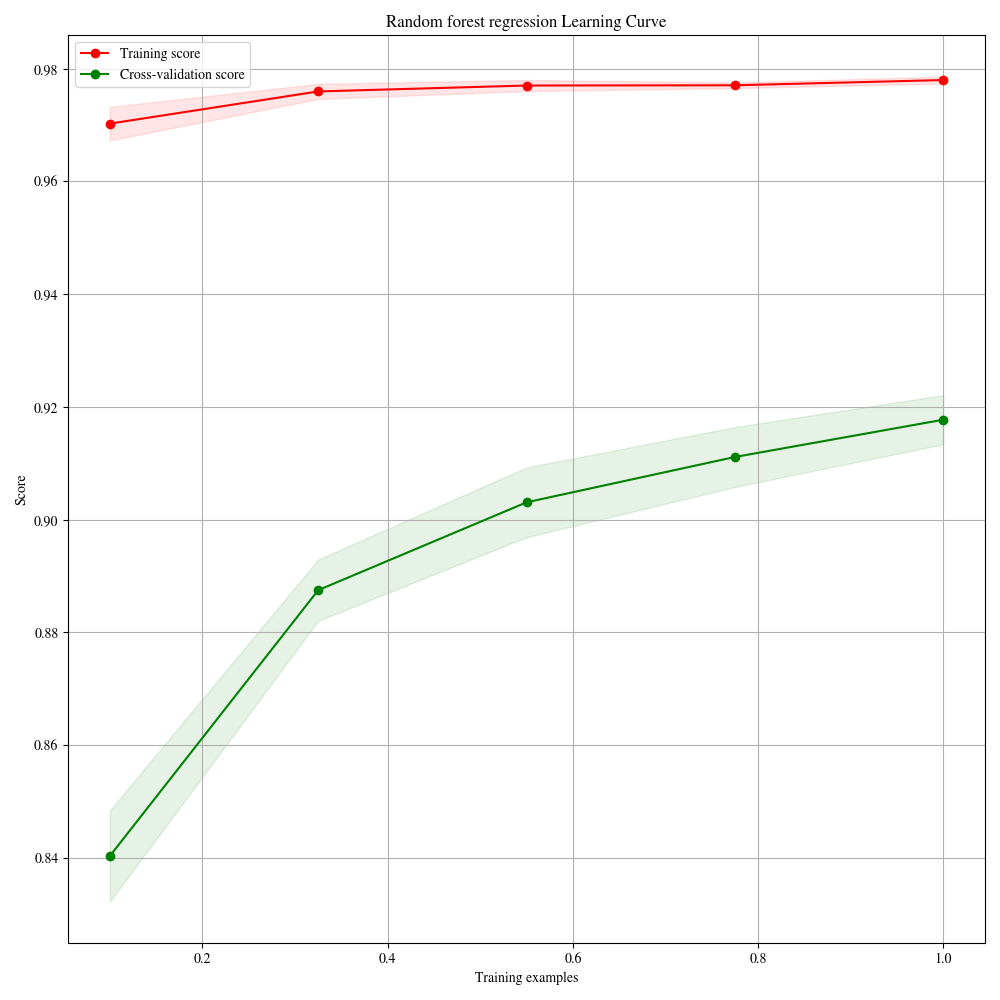
\includegraphics[scale=0.5]{images/randomforestlearningcurve.png}
    \caption{A plot showing the cross validation scores along with training scores for the random forest.}
\end{figure}
\section{Running Instructions}
The project is structured as follows:
    \begin{itemize}
        \item utils/ - containing utilities such as plotting helper functions;
        \item figs/ - the directory where the figures get saved;
        \item data/ - a directory containing the datasets (train, test and original);
        \item describe.py - a script that performs descriptive analytics on the dataset;
        \item evaluate\_models.py - evaluates the trained models;
        \item feature\_selection.py - A script that performs feature selection analysis
    \end{itemize}{}
Listing~\ref{lst:running} shows how to run the scripts.
\begin{listing}[ht]
\label{lst:running}
\begin{minted}[linenos, breaklines]{sh}
 venv/bin/python <file_name>
\end{minted}
\caption{Running the scripts.}
\end{listing}{}
\paragraph{Dependencies}
\begin{itemize}
    \item Scikit Learn~\autocite{scikitlearn}
    \item Numpy~\autocite{2020SciPyNMeth}
    \item Matplotlib~\autocite{hunter2007matplotlib}
    \item Statsmodels (Used for calculating the variance inflation factor)~\autocite{seabold2010statsmodels}
\end{itemize}{}
\newpage
\printbibliography
\newpage
\begin{appendices}

\end{appendices}
\end{document}
